\documentclass{article}
\usepackage[utf8]{inputenc}
\usepackage{times}
\usepackage{latexsym}
\usepackage{acl2020}
\usepackage{graphicx}

\title{Using Single-Regression BERT to Predict Humor Content}

\author{
James Blackburn (jimbb82@uw.edu)\\
Joshua Valdez (jdv2@uw.edu)\\
Joseph Nollette (nollejos@uw.edu)\\
Christian Kavouras (cdkavour@uw.edu)
}

\date{\vspace{-5ex}}

\begin{document}

\maketitle


\begin{abstract}
We present a system for predicting the humor content of English-language news article headlines; specifically, the boost in perceived humor resulting from the replacement of one word or phrase in the original headline with a new word, as rated by human judges.
\end{abstract}

\section{Introduction}
The SemEval series seeks to expand upon the current state of the art semantic analysis through exploration of various shared tasks. Such tasks allow participants to advance the work done in the field by experimentation through modeling, dataset creation, and the like. SemEval-2020 Task 7 seeks to expand upon the task of predicting the humor content of chunks of text, and attempts to measure the change in human-judged humor values when individual words are replaced. We will build a system that -- given original chunks and edited chunks -- will predict the mean humor score of an edited headline. In addition, we will formulate an adaptation task which uses our learned understanding of humor for a separate task application, analyzing the relative humor of Reddit threads.

\section{Task Description}
The primary task of this project is to implement a regression model to predict the degree of humor of brief news headlines, using data from the Humicroedit data set. This data set contains the text of news headlines in which one word has been edited to change a serious headline into a humorous one. All training instances contain the full text of the headline, the word that was replaced, the new word that was put in its place, and a decimal score between 0 (not funny) and 3 (very funny), obtained by taking the average score given by five human judges. The dataset containing the description of this task and its dataset can be found \href{https://competitions.codalab.org/competitions/20970}{here}.\cite{hossain-etal-2019-president}

For our adaptation task, we apply a similar model, trained on both the original and edited headlines referenced above, to Reddit data scraped from the web. In order to test the applicability of our system to a secondary task, we try to approximate the relative humor of reddit data, to compare with our system's predictions. The goal is to determine whether we can predict the humor content of reddit data using the upvote count on each datum as a proxy for how relatively humorous it might be.

\section{Approach}
To formulate our regression model, we follow the paradigm of pre-training and fine-tuning, using a single-regression, pre-trained BERT (Bidirectional Encoder Representations from Transformers) model. The model is fine-tuned on our headline data and evaluated as a single-regression task with RMSE loss. The availability of external GPUs allows us to fine-tune BERT itself. The model uses raw-sentence embeddings as input which are then tokenized using BertTokenzer. We tune hyper-parameters for the number of epochs trained against and number of batches used in order to converge on the best scoring model.  We use the provided train/dev/test split from the shared task data-set in order to develop and test our model performance.


\section{System Overview}

We use a bidirectional encoder representation from transformers (BERT) model to predict the humor content of edited headlines. This model \cite{DBLP:journals/corr/abs-1810-04805} consists of a series of transformer encoders which takes embeddings of labeled headlines as its input and generates a predictied humor score for each instance.

% \vspace{1cm}
\begin{figure}
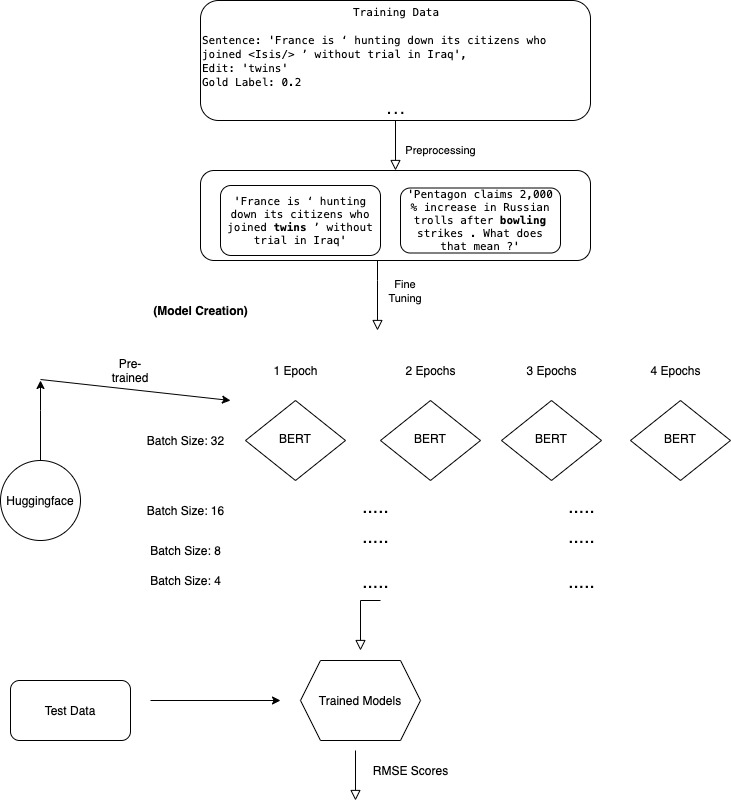
\includegraphics[scale=0.25]{classifier.jpg}
\caption{System Architecture for our primary task prediction}
\end{figure}
% \vspace{1cm}

To complete the pretraining phase, sixteen distinct models were generated from embeddings of the labeled training instances, by varying the number of training epochs from one to four, and employing batch sizes of 4, 8, 16, and 32 instances. A root mean square error is employed as the loss function.


\section{System Improvement}
We have considered various possibilities for the improvement of our primary task, looking to the literature for insight regarding our choice. Ultimately, we decided on an attempt to fine tune further using a feed-forward neural network. We use this FFNN as a head on top of our highest scoring BERT model, and fine-tune on our development set (without further tuning of BERT itself).  We adjusted five parameters along three values each to tune the model, including learning-rate, dropout, number of epochs trained, number of hidden layers, and batch-size, in order to find the highest scoring values.

\section{Adaptation Task}
We aimed to investigate the performance of the BERT model's humor prediction capabilities on another data source with similarities to the original headline dataset.

Reddit post titles offer abundance, diversity of content, and degree of brevity similar in scale to news headlines. With this motivation in mind, we built a simple scraper using Python's praw library to gather the top 1,000 posts of all time from twelve subreddits. Of these, six were understood by users to feature content that was humorous, such as jokes and witticisms, while the other six were meant for non-humorous content such as current events and sports.

While there is no gold standard for the humor content of Reddit posts, we chose to explore other ways of quantifying their humor content using our model. One possible metric to be used as a proxy for a humor content score was the \textit{upvote score} of each post -- our hypothesis, essentially, was that high-scoring posts from humorous subreddits would show higher humor scores than not only low-scoring posts from the humorous subreddits, but also similar-scoring posts from non-humorous subreddits (i.e. high-scoring posts from news subreddits are assumed not to be highly-rated because they are funny).

After obtaining the roughly 12,000 posts and their upvote scores, separated by subreddit, we sought to pre-process our data to achieve an even distribution of upvote scores. To this end, we plotted upvote score count across each thread to see the resulting distribution, and found all distributions to be left skewed. To remedy this, use only the bottom half of each distribution, the subset of which we found to be distinctly linear. We then normalized the upvote scores of the remaining data to a range from 0.0 to 3.0, in order to flatten out extreme outliers among upvote scores and distribute the post scores so as to conform approximately to the scale used in our primary task. The post titles were then fed into our model and given a predicted humor score.

To quantify the presence or absence of such a relationship, we calculated the Spearman correlation of predicted humor and upvote score for each post in each subreddit. 

\section{Results}

\subsection{Primary Task Results}

Below is a table of the RMSE values for the sixteen combinations of epochs and batch size for the primary task. Our Baseline value was formulated using the RMSE across the label values of our training and test data.\\
\\
baseline: 0.57471

\begin{center}
\begin{tabular}{|c|c|c|c|c|}
\hline
epochs & bs=32 & bs=16 & bs=8 & bs=4 \\
\hline
1 & 0.54199 & 0.54312 & 0.53396 & 0.53438 \\
2 & 0.53324 & 0.54381 & 0.5383 & 0.54047 \\
3 & 0.54728 & 0.54737 & 0.56014 & 0.55393 \\
4 & 0.55964 & 0.55747 & 0.56742 & 0.56569 \\
\hline
\end{tabular}
\end{center}

As shown, the best result we have obtained from this initial run is from 2 epochs and a batch size of 32.

\subsection{System Improvement Results}

Our attempts to improve the original BERT model with a neural network head involved testing all combinations of the hyperparameters described in section 5, yielding 243 (3\^5) distinct trials, the best three of which are shown below:

\begin{center}
\begin{tabular}{|c|c|c|c|c|c|}
\hline
RMSE & epoch & bs & learn & drop & hl \\
\hline
0.56156 & 8 & 4 & 2E-4 & 0.4 & 2 \\
0.5634 & 8 & 4 & 2E-4 & 0.4 & 1 \\
0.56541 & 4 & 8 & 2E-4 & 0.2 & 2 \\
\hline
\end{tabular}
\end{center}

While these remain below the original baseline, none of these attempts improved upon the original best RMSE from our original task.

\subsection{Adaptation Task Results}

Across the board, we were unable to find any sign of correlation between normalized upvote scores and predicted humor scores of reddit data.  The spearman correlation across all 12 sub-reddits are very close to 0, indicating no correlation. Below are two line-graphs plotting up-vote score to predicted humor score for 2 seperate subreddit threads, demonstrating this lack of correlation.



\begin{figure}[h]
\centering
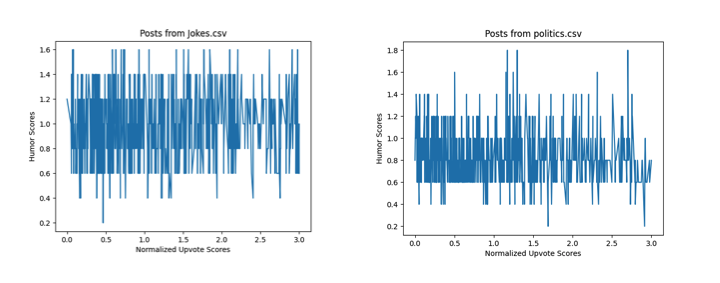
\includegraphics[width=.5 \textwidth]{correlation_comparison.png}
\caption{Graphical plot of normalized up-vote score to humor score; on the left, scores for a humorous subreddit (Jokes), and on the right, scores for a non-humorous thread (Politics)}
\end{figure}

\section{Discussion}

While our methods did not discover any quantifiable correlation between upvote scores and humor content as predicted by our initial system, these results do reveal potentially promising avenues for future research.

We employed a method of normalizing reddit scores to our existing 0 to 3 scale of humor. This was motivated mainly by two observations: first, the curve of upvote scores in any given subreddit, as plotted against rank, was fairly linear when extreme outliers were pruned from the dataset. Second, the upvote scores of posts within a given subreddit vary quite dramatically depending on the relative popularity of the subreddit -- for example, the top all-time post of r/oneliners had a score of 1,985, while the top all-time post of r/news had a score of 365,120. While we feel that our motivation for addressing these issues was well-informed, it is likely that doing so resulted in a loss of important information.

These results also encourage discussion around the basic differences between the nature of the primary task and the adaptation task. While the primary task involved a well-defined procedure for building a human-scored gold standard, our approach to the adaptation task was admittedly rather experimental, operating on the hypothesis that reddit users in humorous subreddits are essentially doing the same work as the primary task's human judges when they boost the score of a given post. The lack of correlation demonstrates that this hypothesis, while reasonable on its surface, does not hold true, and raises further questions about the various ways text-based humor can be expressed across different media.

\section{Future Improvements}
While our prediction system is achieves fair results, there is certainly room for improvement.
The system could benefit from more refined methods of fine-tuning, including, but not limited to, ensemble methods, more hand-crafted data, or augmented data (possibly variations on transfer learning from other shared tasks).
As for our adaptation task, the system could potentially benefit from human-valued annotations for reddit data, which would allow us to verify whether our null results are a result of the in-accuracy of our system predictions, or simply due to a lack of correlation to upvoting. An additional improvement in the absence of such data would be to use predictions for humor scores for additional reddit data as silver (noisy) labels, which could be fed back into our regression model system for supplemental training.

\section{Conclusion}

A single-regression BERT model performs quite well at predicting the humor content of human-scored news headlines. However, when applied to reddit posts that performed well in humorous subreddits, our methods yielded no quantifiable correlation between the post's upvote score and its predicted humor content.

\section{Works Cited}
\begin{itemize}
\item BERT paper: (Devlin et al., 2018) https://arxiv.org/pdf/1810.04805.pdf
\item Aspect-based sentiment analysis - ideas from a similar task domain (Xu, et al., 2019) https://arxiv.org/pdf/1904.02232.pdf
\item Winning Model for same task (Spanish Dataset) http://ceur-ws.org/Vol-2421/HAHA\_paper\_3.pdf
\end{itemize}

\bibliographystyle{acl_natbib}
\bibliography{refs}

\end{document}
